% Drawing 154/06-30 -- folder 154, batch 06, archive page 113 (PDF page 114).
% Transcription: au-dessous, au crayon, un huit (deux cercles tangents) traversé de courbes, et à côté le même huit en couleur, vert clair et vert foncé, des arcs renforcés en brun et marqués de petits traits rouges
% Kind: figure-eight in pencil and in colour. Method 2 (schematic redraw from the facsimile). Status: partial.
% Notes: Pencil eight: two tangent circles, three curves fanning across the upper one from its top to the tangency point and beyond, one curve down the lower one. Coloured eight: the two circles dark green on the left and light green on the right, seven short arcs thickened in brown (top, upper left, right, at the tangency, lower right, lower left, bottom), five green points on the upper circle. The small red ticks on the brown arcs are not drawn; the brown arcs are placed approximately. Redrawn 2026-11-12 (issue 128): to check again.
% Coordinates: 1 unit = 1 mm = 1/100 of the crop width (bbox in page fractions: [0.56, 0.29, 0.89, 0.5]).
% Redrawn by Claude (claude-fable-5-2), issue #128, 2026-11-12; not checked by a human; not compiled (no TeX in the session).
% Rights: reproduces part of the work -- behind RENDER_TRANSCRIPTS, never published by itself.
\documentclass[tikz,border=3pt]{standalone}
\usepackage{amsmath,amssymb}
\usetikzlibrary{patterns,arrows.meta}
\tikzset{Lg/.style={green!60!black!70}, Dg/.style={green!45!black}, Br/.style={brown!80!black}, pencil/.style={black!45}, struck/.style={black!35}, mpt/.style={circle,draw,inner sep=1.3pt}, pt/.style={circle,fill,inner sep=0.9pt}, opt/.style={circle,draw,fill=white,inner sep=1.1pt}}
\begin{document}
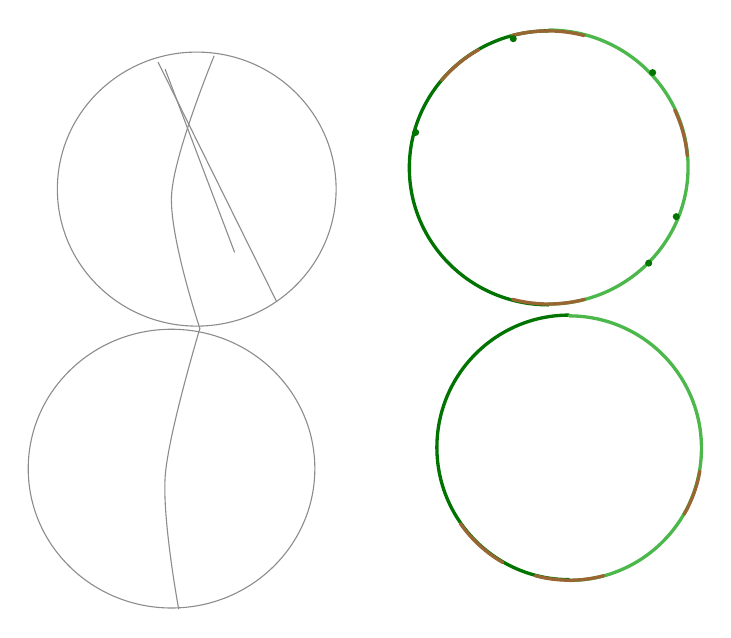
\begin{tikzpicture}[x=1mm,y=1mm,line cap=round,line join=round,font=\scriptsize]
\draw[pencil] (25.4,-29.4) ellipse[x radius=17.7, y radius=17.4];
\draw[pencil] (22.2,-64.9) ellipse[x radius=18.2, y radius=17.7];
\draw[pencil] (20.5,-13.3) -- (35.5,-43.6);
\draw[pencil] plot[smooth, tension=0.55] coordinates {(27.6,-12.5) (22.2,-30.2) (25.8,-47.1)};
\draw[pencil] (21.4,-14.2) -- (30.2,-37.4);
\draw[pencil] plot[smooth, tension=0.55] coordinates {(25.8,-47.1) (21.4,-65.8) (23.1,-82.7)};
\draw[Dg,very thick] (70.1,-9.3) arc[start angle=90, end angle=270, x radius=17.7, y radius=17.4];
\draw[Lg,very thick] (70.1,-44) arc[start angle=-90, end angle=90, x radius=17.7, y radius=17.4];
\draw[Dg,very thick] (72.7,-45.4) arc[start angle=90, end angle=270, x radius=16.8, y radius=16.8];
\draw[Lg,very thick] (72.7,-79.1) arc[start angle=-90, end angle=90, x radius=16.8, y radius=16.8];
\draw[Br,very thick] (74.6,-9.9) arc[start angle=75, end angle=105, x radius=17.7, y radius=17.4];
\draw[Br,very thick] (61.2,-11.7) arc[start angle=120, end angle=140, x radius=17.7, y radius=17.4];
\draw[Br,very thick] (87.7,-25.2) arc[start angle=5, end angle=25, x radius=17.7, y radius=17.4];
\draw[Br,very thick] (65.5,-43.4) arc[start angle=255, end angle=285, x radius=17.7, y radius=17.4];
\draw[Br,very thick] (87.3,-70.7) arc[start angle=-30, end angle=-10, x radius=16.8, y radius=16.8];
\draw[Br,very thick] (58.9,-71.9) arc[start angle=215, end angle=240, x radius=16.8, y radius=16.8];
\draw[Br,very thick] (68.4,-78.5) arc[start angle=255, end angle=285, x radius=16.8, y radius=16.8];
\node[pt,Dg] at (65.6,-10.3) {};
\node[pt,Dg] at (83.3,-14.6) {};
\node[pt,Dg] at (53.2,-22.2) {};
\node[pt,Dg] at (86.3,-32.9) {};
\node[pt,Dg] at (82.8,-38.8) {};
\end{tikzpicture}
\end{document}
